%%%%%%%%%%%%%%%%%%%%%%%%%%%%%%%%%%%%%%%%%%%%%%%%%%%%%%%%%%%%%%%%%%%%%%
% Lớp 11 | Dãy số. Cấp số cộng. Cấp số nhân | Dãy số
% Dạng 1D2?1-6: Toán thực tế áp dụng dãy số
% Số câu: 25  (sinh tự động bởi tach_cau.py; từ nay thầy sửa trực tiếp file này)
%%%%%%%%%%%%%%%%%%%%%%%%%%%%%%%%%%%%%%%%%%%%%%%%%%%%%%%%%%%%%%%%%%%%%%

%%%%%%%%%%%%%%%% ĐÚNG/SAI %%%%%%%%%%%%%%%%

% nguồn: Ok_dungsai_lop11_Lan2
\begin{ex}%[1D2V1-6]%[ma:de4cfed3]
	Vi khuẩn E. Coli sinh sản thông qua một quá trình gọi là quá trình phân đôi. Vi khuẩn E. Coli phân chia làm đôi cứ sau $20$ phút. Giả sử tốc độ phân chia này được duy trì trong $12$ giờ kể từ khi vi khuẩn ban đầu xâm nhập vào cơ thể. Biết ban đầu có $1$ vi  khuẩn E. Coli.
	\choiceTF 
		{Sau $1$ giờ, số  lượng vi khuẩn là $6$ con}
		{\True Sau $2$ giờ, số  lượng vi khuẩn là $64$ con}
		{Sau $12$ giờ, số lượng vi khuẩn là $2^{12}$ con} 
		{\True Giả sử có một nguồn dinh dưỡng vô hạn để vi khuẩn E. Coli duy trì tốc độ phân chia như cũ trong $48$ giờ kể từ khi vi khuẩn ban đầu xâm nhập vào cơ thể. Sau $48$  giờ, số lượng vi khuẩn là $2^{144}$ con}
	\loigiai{ 
		Sau $20$ phút lần một, số vi khuẩn  là $1\cdot2=2$ con.\\
		Sau $20$ phút lần hai, số vi khuẩn là  $2\cdot2=2^2$ con.\\
		Sau $20$  phút lần ba, số vi khuẩn là $2^2\cdot2=2^3$ con.\\
		 $\cdots$\\
		Sau  $20$ phút lần $n$, số vi khuẩn là $2^n$ con.
		\begin{itemchoice}
			\itemch \textbf{Sai.}\\ 
			Sau $1$ giờ, số lượng  vi khuẩn là $2^3=8$ con.
			\itemch \textbf{Đúng.}\\ 
			Sau $2$ giờ, số lượng  vi khuẩn là $2^6=64$ con.
			\itemch  \textbf{Sai.}\\
			Sau $12$ giờ, số lượng vi khuẩn  là $2^{36}$ con.
			\itemch \textbf{Đúng.}\\ 
			Sau $24$ giờ, số lượng vi khuẩn là  $2^{144}$ con.
		\end{itemchoice}
	 }
\end{ex}

% nguồn: Ok_dungsai_lop11_Lan2
\begin{ex}%[1D2V1-6]%[ma:1e37e2c0]
	Bà Hoa gửi vào một ngân hàng số tiền $200$ triệu đồng với lãi suất $5\%$ một năm theo hình thức  lãi kép, kì hạn $1$ tháng. Số tiền(triệu đồng) của bà Hoa sau $n$ tháng được tính theo công thức $T_n=200\left(1+\dfrac{0{,}05}{12}\right)^n$.
	 \choiceTF
		{\True  Sau $1$ tháng, số tiền bà Hoa nhận được là khoảng $200{,}83$ (triệu đồng)}
		{\True Sau $2$ tháng, số tiền  bà nhận được là khoảng $201{,}67$ (triệu đồng)}
		{\True  Sau $14$ tháng, số tiền bà nhận được là khoảng $211{,}99$ (triệu đồng)}
		{Sau $17$  tháng, số tiền bà nhận được là khoảng $215{,}65$ (triệu đồng)}
	\loigiai{\begin{itemchoice}
		\itemch Sau $1$  tháng, số tiền bà Hoa nhận được là $T_1 = 200\left(1+\dfrac{0{,}05}{12}\right)^1 \approx 200{,}83$ (triệu đồng).
		\itemch Sau $2$ tháng, số tiền bà nhận được là $T_2  = 200\left(1+\dfrac{0{,}05}{12}\right)^2 \approx 201{,}67$ (triệu đồng).
		\itemch Sau $14$ tháng, số tiền bà nhận được là $T_{14} = 200\left(1+\dfrac{0{,}05}{12}\right)^{14} \approx 211{,}99$  (triệu đồng).
		\itemch Sau $17$ tháng, số tiền bà nhận được  là $T_{17} = 200\left(1+\dfrac{0{,}05}{12}\right)^{17} \approx 214{,}65$ (triệu đồng).
\end{itemchoice}}
\end{ex}

% nguồn: Ok_dungsai_lop11_Lan2
\begin{ex}%[1D2V1-6]%[ma:ea983e31]
	Giá của một chiếc máy photocopy lúc mới mua là $50$ triệu đồng. Biết rằng giá trị của nó sau mỗi năm sử dụng chỉ còn $75\%$ giá trị trong  năm liền trước đó. Gọi $T_n$ (triệu đồng) là giá trị còn lại của chiếc máy photocopy đó sau $ n$ năm kể từ khi mua.
	 \choiceTF
		{\True  $T_1=37{,}5$ triệu đồng}
		 {\True $T_2=28{,}125$ triệu đồng}
		{$T_4\approx 11{,}87$ triệu  đồng}
		{\True $T_n=50\cdot0{,}75^n$  triệu đồng}
	 \loigiai{
		\begin{itemchoice}
			 \itemch \textbf{Đúng.}\\
			Giá trị của máy photocopy sau $1$ năm sử dụng là $T_1=50\cdot0{,}{75^1}=37{,}5$ triệu  đồng.
			 \itemch \textbf{Đúng.}\\
			Giá trị của  máy photocopy sau $2$ năm sử dụng là $T_2=T_1\cdot0{,}75=50\cdot0{,}75^{2}=28{,}125$.
			 \itemch \textbf{Sai.}\\
			Giá trị  của máy photocopy sau $3$ năm sử dụng là $T_3=T_2\cdot0{,}75=50\cdot0{,}75^3$ triệu đồng.\\
			 Giá trị của máy photocopy sau $4$ năm sử dụng là $T_4=T_3\cdot0{,}75=50\cdot0{,}75^4\approx 15{,}82$ triệu đồng.
			 \itemch \textbf{Đúng.}\\
			Tổng quát, giá trị của máy photocopy sau $n$ năm sử dụng là $T_n=50\cdot0{,}75^n$ triệu đồng. 
		\end{itemchoice}
	} 
\end{ex}

% nguồn: Ok_dungsai_lop11_Lan2
\begin{ex}%[1D2V1-6]%[ma:78e5a16e]
	Bà Hoa gửi vào một ngân hàng số tiền $200$ triệu đồng với lãi suất $5 \%$ một năm theo hình thức lãi kép,  kì hạn $1$ tháng. Số tiền (triệu đồng) của bà Hoa sau $n$ tháng được tính theo công thức $T_n=200\left(1+\dfrac{0{,}05}{12}\right)^n$. Khi đó:
	 \choiceTF
		{\True Sau $1$ tháng,  số tiền bà Hoa nhận được là khoảng $200{,}83$ (triệu đồng)}
		{\True Sau $2$ tháng, số tiền bà nhận được là  khoảng $201{,}67$ (triệu đồng)}
		{\True Sau $14$ tháng, số tiền bà nhận được là khoảng $211{,}99$ (triệu đồng)} 
		{Sau $17$  tháng, số tiền bà nhận được là khoảng $215{,}65$ (triệu đồng)}
	\loigiai{ 
		\begin{itemchoice}
			 \itemch \textbf{Đúng.}\\
			Sau $1$ tháng, số  tiền bà Hoa nhận được là $T_1=200\left(1+\dfrac{0{,}05}{12}\right)^1 \approx 200{,}83$ (triệu đồng).
			\itemch  \textbf{Đúng.}\\
			Sau $2$ tháng, số tiền bà Hoa nhận được là $T_2=200\left(1+\dfrac{0{,}05}{12}\right)^2 \approx 201{,}67$ (triệu  đồng).
			\itemch  \textbf{Đúng.}\\
			 Sau $14$ tháng, số tiền bà Hoa nhận được là $T_{14}=200\left(1+\dfrac{0{,}05}{12}\right)^{14} \approx 211{,}99$ (triệu đồng).
			 \itemch \textbf{Sai.}\\
			Sau $17$ tháng, số tiền bà Hoa nhận được  là $T_{17}=200\left( 1+\dfrac{0{,}05}{12} \right)^{17}\approx 214{,}65$ (triệu đồng).
		\end{itemchoice}
	} 
\end{ex}


%%%%%%%%%%%%%%%% TRẢ LỜI NGẮN %%%%%%%%%%%%%%%%

% nguồn: Ok_TraLoiNgan_Lop11_Lan1
\begin{ex}%[1D2H1-6]%[ma:981ed317]
	Một công ty dược phẩm đang thử nghiệm một loại thuốc  mới. Một thí nghiệm bắt đầu với $1{,}0 \cdot 10^9$ vi khuẩn. Một liều thuốc được sử dụng sau mỗi bốn giờ có thể tiêu diệt $4{,}0 \cdot 10^8$ vi khuẩn. Giữa các liều thuốc, số lượng vi khuẩn tăng lên $25 \%$. Tìm số vi khuẩn còn sống trước lần sử dụng thuốc thứ năm (đơn vị triệu con) (kết quả làm tròn đến hàng đơn vị).
	\shortans{135} 
	\loigiai{ 
		Gọi $u_1=1{,}0 \cdot 10^9$ là số vi khuẩn tại thời điểm ban đầu và $u_n$ là số vi khuẩn trước lần dùng thuốc thứ $n$.\\ 
		Do mỗi liều thuốc được sử  dụng sau bốn giờ có thể tiêu diệt $4{,}0 \cdot 10^8$ vi khuẩn và giữa các liều thuốc, số lượng vi khuẩn tăng lên $25 \%$ nên ta có
		$$ 
		u_{n+1}=(u_n-4{,}0 \cdot  10^8)+25 \% \cdot u_n=1{,}25 u_n-4{,}0 \cdot 10^8.
		$$ 
		Ta có  hệ thức truy hồi $u_1=1{,}0 \cdot 10^9$; $u_{n+1}=1{,}25 u_n-4{,}0 \cdot 10^8$.
		$$ 
		\begin{aligned}
			& u_1=1{,}0 \cdot  10^9; \\
			& u_2=1{,}25 u_1-4{,}0 \cdot 10^8=1{,}25 \cdot 1{,}0 \cdot 10^9-4{,}0  \cdot 10^8=8{,}5 \cdot 10^8; \\
			& u_3=1{,}25 u_2-4{,}0 \cdot 10^8=1{,}25 \cdot 8{,}5 \cdot 10^8-4{,}0 \cdot 10^8=6{,}625 \cdot  10^8; \\
			& u_4=1{,}25 u_3-4{,}0 \cdot 10^8=1{,}25 \cdot 6{,}625 \cdot 10^8-4{,}0 \cdot 10^8=4{,}28125 \cdot 10^8;  \\
			& u_5=1{,}25 u_4-4{,}0 \cdot 10^8=1{,}25  \cdot 4{,}28125 \cdot 10^8-4{,}0 \cdot 10^8=1{,}3515625 \cdot 10^8=135\,156\,250.
		\end{aligned}
		 $$
	Vậy số vi khuẩn còn sống trước lần sử dụng thuốc thứ năm là $135\,156\,250\approx 135$  (triệu) con.}
\end{ex}

% nguồn: Ok_TraLoiNgan_Lop11_Lan2
\begin{ex}%[1D2H1-6]%[ma:9d77c902]
	Bác Thanh gửi tiết kiệm $200$ triệu đồng kì hạn $1$ tháng với lãi suất $6{,}5\%$ một năm theo hình thức  lãi kép. Số tiền của bác Thanh thu được sau $n$ tháng được cho bởi công thức $A_n=200\left( 1+\dfrac{0{,}065}{12} \right)^n$. Tính số tiền lãi bác Thanh nhận được sau $7$ tháng theo đơn vị triệu đồng (làm tròn đến hàng phần trăm).
	 \shortans{7,71}
	\loigiai{ 
		Ta  có:\\
		Số tiền bác Thanh nhận được sau  $8$ tháng là $A_7=200\left(1+\dfrac{0{,}065}{12}\right)^7=207{,}71$.\\
		Số tiền lãi  bác Thanh nhận được sau $7$ tháng là $207{,}71-200=7{,}71$.
	} 
\end{ex}

% nguồn: Ok_TraLoiNgan_Lop11_Lan2
\begin{ex}%[1D2H1-6]%[ma:9f30cfc5]
	Bác Thanh gửi tiết kiệm $200$ triệu đồng kì hạn $1$ tháng với lãi suất $6{,}5\%$ một năm theo hình thức lãi kép. Số tiền của bác Thanh thu được sau $n$ tháng được cho bởi  công thức $A_n=200\left( 1+\dfrac{0{,}065}{12} \right)^n$. Bác Thanh cần gửi ít nhất bao nhiêu tháng để nhận được số tiền cả gốc và lãi là $208{,}81$ triệu đồng.
	 \shortans{8}
	\loigiai{ 
		Số tiền bác Thanh nhận được sau $n$ tháng là $A_n=200\left( 1+\dfrac{0{,}065}{12} \right)^n=208{,}81$.\\ 
		Suy ra $n  \approx 8$. Vậy bác Thanh cần gửi ít nhất $8$ tháng.
	} 
\end{ex}

% nguồn: Ok_TraLoiNgan_Lop11_Lan2
\begin{ex}%[1D2H1-6]%[ma:79acfadf]
	Ông An gửi tiết kiệm $100$ triệu đồng kì hạn $1$ tháng với lãi suất $6\%$ một năm theo hình thức tính lãi  kép. Số tiền của ông An thu được sau $n$ tháng được cho bởi công thức $A_n=100\left(1+\dfrac{0{,}06}{12} \right)^n$. Tìm số tiền ông An nhận được sau $1$ năm theo đơn vị triệu đồng (làm tròn đến hàng triệu).
	\shortans{106} 
	 \loigiai{
		 Số tiền ông An nhận được sau $1$ năm là $A_{12}=100\left( 1+\dfrac{0{,}06}{12} \right)^{12} \approx 106$ triệu đồng.
	} 
\end{ex}

% nguồn: Ok_TraLoiNgan_Lop11_Lan2
\begin{ex}%[1D2H1-6]%[ma:4a087a2a]
	Một người gửi $100$ triệu đồng vào ngân hàng với kì hạn $3$ tháng, lãi suất $5\%$ một quý theo hình thức lãi kép. Sau đúng $6$ tháng người đó gửi thêm $100$ triệu đồng với  hình thức và lãi suất như trên. Hỏi sau đúng một năm tính từ lần gửi đầu tiên người đó nhận được bao nhiêu tiền theo đơn vị triệu đồng, làm tròn đến hàng đơn vị?
	 \shortans{232}
	 \loigiai{
		Sau đúng $6$ tháng  người đó thu được số tiền cả vốn lẫn lãi là $M_1=100\left( 1+5\% \right)^2$.\\
		Sau một năm tính từ lần gửi đầu tiên  người đó nhận được cả vỗn lẫn lãi là
		\begin{equation*}
			M_2=\left( 100+M_1  \right)\left( 1+5\% \right)^2 \approx 232.
		\end{equation*}
	} 
\end{ex}

% nguồn: Ok_TraLoiNgan_Lop11_Lan2
\begin{ex}%[1D2H1-6]%[ma:d750a155]
	Bác Thanh gửi tiết kiệm $A$ triệu đồng kì hạn $1$ tháng với lãi suất $6{,}5\%$ một năm theo hình thức lãi kép. Số tiền của bác  Thanh thu được sau $n$ tháng được cho bởi công thức $A_n=A\left( 1+\dfrac{0{,}065}{12} \right)^n$. Hỏi bác Thanh cần gửi vào ngân hàng số $A$ là bao nhiêu triệu đồng để sau $4$ tháng bác Thanh nhận được $204{,}37$ triệu đồng (làm tròn kết quả đến hàng đơn vị).
	 \shortans{200}
	\loigiai{ 
		Số tiền bác Thanh nhận  được sau $4$ tháng là $A_4=A\left(1+\dfrac{0{,}065}{12}\right)^4=204{,}37$.\\
		 $A = 204{,}37 : \left(1+\dfrac{0{,}065}{12}\right)^4 \approx 200$ triệu đồng.\\
		$A=200$. 
	} 
\end{ex}

% nguồn: Ok_TraLoiNgan_Lop11_Lan2
\begin{ex}%[1D2H1-6]%[ma:a0f3daa4]
	Bác Thanh gửi tiết kiệm $200$ triệu đồng kì hạn $1$ tháng với lãi suất $6{,}5\%$ một năm theo hình thức lãi kép. Số tiền của bác Thanh thu được sau $n$ tháng được cho bởi công thức $A_n=200\left( 1+\dfrac{0{,}065}{12}  \right)^n$. Tính số tiền bác Thanh nhận được sau $3$ tháng theo đơn vị triệu đồng (làm tròn đến hàng đơn vị).
	 \shortans{203}
	 \loigiai{
		Ta có số tiền bác Thanh  nhận được sau $3$ tháng là $A_3=200\left( 1+\dfrac{0{,}065}{12} \right)^3=203{,}27$.
	} 
\end{ex}

% nguồn: Ok_TraLoiNgan_Lop11_Lan2
\begin{ex}%[1D2H1-6]%[ma:dc9b883e]
	Một người lần đầu gửi vào ngân hàng $100$ triệu đồng với kì hạn $3$ tháng, lãi suất $2\%$ một quý. Biết rằng nếu không rút  tiền ra khỏi ngân hàng thì cứ sau mỗi quý số tiền lãi sẽ được nhập vào gốc để tính lãi cho quý tiếp theo. Sau đúng $6$ tháng, người đó gửi thêm $100$ triệu đồng với kỳ hạn và lãi suất như trước đó. Tổng số tiền người đó nhận được $1$ năm sau khi gửi tiền theo đơn vị triệu đồng?
	 \shortans{212}
	 \loigiai{
		Số tiền nhận về sau $6$ tháng của $100$ triệu gửi trước là $M_1 =  100\left( 1+2\% \right)^2$ triệu.\\
		Số tiền nhận về sau $1$  năm là $M_2 = (100+M_1)(1+2\%)^2$\\
		Vậy tổng số tiền là $M_2=212{,}283216 \approx 212$ triệu. 
	 }
\end{ex}

% nguồn: Ok_TraLoiNgan_Lop11_Lan1
\begin{ex}%[1D2V1-6]%[ma:ec9f9002]
	Vào đầu mỗi tháng, ông An đều gửi vào ngân hàng số tiền cố định $30$ triệu đồng  theo hình thức lãi kép với lãi suất $0{,}6 \%$/tháng. Gọi $A$ (triệu đồng) là số tiền ông An có được sau tháng thứ hai. Tính $A$ (làm tròn đến hàng đơn vị)
	 \shortans{61.}
	 \loigiai{
		 Số tiền ông An có được
		\begin{itemize}
			\item Sau tháng thứ nhất là  $T_{1} =30+30\cdot \dfrac{0,6}{100} =30\left(1+\dfrac{0,6}{100} \right)=30,18$ (triệu đồng).
			\item Sau tháng  thứ hai là\\
			$T_{2} =30+30\left(1+\dfrac{0,6}{100} \right)+\left[30+30\left(1+\dfrac{0,6}{100}  \right)\right]\cdot\dfrac{0,6}{100} \approx 60{,}54$ (triệu đồng).
	\end{itemize}}
\end{ex}

% nguồn: Ok_TraLoiNgan_Lop11_Lan1
\begin{ex}%[1D2V1-6]%[ma:e9db14b6]
	Ông Năm vay mượn ngân hàng $200$ triệu đồng với lãi suất $6\%$/năm. Ông đồng ý trả theo kì hạn $5$ triệu đồng mỗi tháng. Hỏi số tiền mà ông Năm còn nợ ngân hàng sau $1$ năm nhiều hơn so  với số tiền ông Năm còn nợ ngân hàng sau $3$ năm là bao nhiêu triệu đồng (làm tròn đến hàng đơn vị)? Biết công thức tính số tiền nợ còn lại sau thời gian $n$ là $u_n=N(r+1)^n-\dfrac{A}{r}[(r+1)^n-1]$, với $N$ là số tiền nợ ban đầu, $r$ là lãi suất theo chu kì, $n$ là thời gian trả nợ theo đơn vị của lãi suất, $A$ là số tiền trả nợ theo kì hạn.
	 \shortans{108}
	\loigiai{ 
		Lãi suất  $r=6\%$/năm $=0,5\%$/tháng.\\
		Số tiền ông Năm nợ ban đầu là $N=200$ triệu  đồng.\\
		Số tiền trả theo kì  hạn là $A=5$ triệu đồng.\\
		 Thời gian trả nợ của ông Năm là $n$ (tháng).\\
		Số tiền ông  Năm còn nợ sau $n$ tháng là\\ $u_n=200(0{,}5\%+1)^n=\dfrac{5}{0{,}5\%}[(0{,}5\%+1)^n-1]$.\\
		Số tiền ông Năm còn  nợ sau $12$ tháng ($1$ năm) là \\
		${{u}_{12}}=200{{\left( 0{,}5\%+1 \right)}^{12}}-\dfrac{5}{0{,}5\%}\left[{{\left( 0{,}5\%+1 \right)}^{12}}-1  \right]\approx 151$ (triệu đồng).\\
		Số tiền ông Năm còn nợ sau  $36$ tháng ($3$ năm) là \\
		${{u}_{36}}=200{{\left( 0{,}5\%+1 \right)}^{36}}-\dfrac{5}{0{,}5\%}\left[{{\left(  0{,}5\%+1 \right)}^{36}}-1 \right]\approx 43$ (triệu đồng).\\
		Số tiền mà ông Năm còn nợ  ngân hàng sau $1$ năm nhiều hơn so với số tiền ông Năm còn nợ ngân hàng sau $3$ năm là $151-43=108$ triệu đồng.
	} 
\end{ex}

% nguồn: Ok_TraLoiNgan_Lop11_Lan1
\begin{ex}%[1D2V1-6]%[ma:5abce922]
	Người ta nuôi cấy $5$ con vi khuẩn ecoli trong  môi trường nhân tạo. Cứ $30$ phút thì vi khuẩn ecoli sẽ nhân đôi $ 1 $ lần.
	Tính số lượng vi khuẩn  thu được sau $3$ lần nhân đôi.
	\shortans{40} 
	\loigiai{ 
		Đặt $u_1=5$, gọi số vi  khuẩn sau $n$ lần phân chia là $u_{n+1}$, khi đó ta có dãy số $(u_n)$: $$u_1=5, \; u_{n+1}=2u_n$$
		Ta có $u_2=2u_1=10$, $u_3=2u_2=20$,  $u_4=2u_3=40$.\\
		Vậy nên sau 3 lần nhân đôi thi  số vi khuẩn là $u_4=40$.
	} 
\end{ex}

% nguồn: Ok_TraLoiNgan_Lop11_Lan1
\begin{ex}%[1D2V1-6]%[ma:d730daf2]
	\immini[thm]{Một chồng cột gỗ được xếp thành các lớp, hai lớp liên tiếp hơn kém nhau $1$ cột gỗ (Hình vẽ minh họa). Gọi $u_n$ là số cột gỗ nằm ở lớp thứ $n$ tính từ trên xuống và cho biết lớp trên cùng có $14$ cột gỗ. Hãy xác định số cột gỗ ở hàng  thứ $20$?
	 \shortans{33}
	}{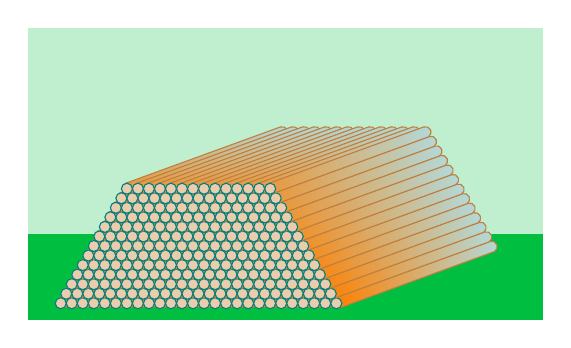
\begin{tikzpicture}[font=\footnotesize,line join=round,line cap=round,>=stealth,scale=0.35]
		 \def\r{0.2}
		\def\n{25} 
		 \def\g{110}
		\fill[teal!50!green](-6*\r,-3*\r) rectangle (3.5*\n*\r,0.5*\n*\r); 
		\fill[teal!50!green,opacity=0.25](3.5*\n*\r,3*\r) rectangle (-6*\r,2*\n*\r); 
		\foreach \j  in {0,...,12}{
			 \pgfmathsetmacro{\m}{\n-\j}
			\foreach \i in{0,...,\m}{ 
			\fill[left color=orange,right color=teal!30,draw=brown](2*\i*\r,0)++(60:2*\j*\r)++(\g:\r)--++(\g-90:6)  arc (\g:-60:\r)--++(\g-270:6)--cycle;
			\fill[orange!20!brown!40,draw=teal](2*\i*\r,0)++(60:2*\j*\r) circle (\r); 
		 }
		} 
	\end{tikzpicture}
	 }
	\loigiai{ 
		\begin{itemize}
			\item Theo giả  thiết ta có công thức truy hồi là $\heva{&u_1=14\\&u_{n+1}=u_n+1.}$
			\item Dùng phương pháp quy nạp  toán học chứng minh được $u_n=13+n$.
			\item  Khi đó hàng thứ $20$ sẽ có $u_{20}=13+20=33$ (cột gỗ).
		\end{itemize}
	} 
\end{ex}

% nguồn: Ok_TraLoiNgan_Lop11_Lan2
\begin{ex}%[1D2V1-6]%[ma:8226fa01]
	Để chuẩn bị cho việc mua nhà, chị An thực hiện việc tiết kiệm bằng cách mỗi tháng gửi đều đặn vào ngân hàng $20$ triệu đồng/tháng. Biết rằng trong thời gian chị An gửi tiền thì ngân hàng áp dụng mức lãi suất $0{,}65$\% tháng và chị An không rút lãi lần nào. Hỏi chị An phải gửi tối thiểu bao nhiêu tháng để có được số tiền $100$ triệu đồng bao gồm cả tiền gốc và  tiền lãi?
	 \shortans{5}
	\loigiai{ 
		Chị An hàng tháng gửi vào ngân hàng một số tiền như nhau là  $A$ đồng, kì hạn $1$ tháng với lãi suất $r\%$ một tháng.\\
		Cuối tháng thứ $1$, chị An có số tiền là \[P_1=A+A  \cdot r=A (1+r).\]
		Đầu tháng thứ $2$, chị An có số  tiền là
		\[P_1+A=A(  1+r)+A=A+A( 1+r)=A[1+( 1+r)]\]
		Cuối tháng thứ $2$, chị An  có số tiền là
		\[P_2=P_1+P_1  \cdot r=A+A( 1+r)+[A+A( 1+r)] \cdot r=A [( 1+r)^2+(1+r)]\]
		Đầu tháng thứ $3$, chị An có số tiền là 
		\[P_2+A=A[(  1+r)+( 1+r)^2]+A=A[1+( 1+r)+( 1+r)^2]\]
		Cuối tháng thứ  $3$, chị An có số tiền là
		\[P_3=P_2+P_2\cdot r=A[1+( 1+r)+( 1+r)^2]+A[1+( 1+r)+( 1+r)^2] \cdot r=A [( 1+r)^3+( 1+r)^2+( 1+r)].\] 
		 $\ldots$\\
		Cuối tháng thứ $n$, chị An có  số tiền là
		\[P_n=A\left[\underbrace{\left( 1+r \right)^n+{{\left( 1+r  \right)}^{n-1}}+{{\left( 1+r \right)}^{n-2}}+....+{{\left( 1+r \right)}^{2}}+\left( 1+r \right)}_{S_n} \right]=A\left( 1+r \right)\dfrac{\left( 1+r \right)^n-1}{r}.\]
		trong đó $A=20$, $r=0{,}65\%$ và $n$ là  số tháng gửi.\\
		Theo giả thiết $P_n=100\Leftrightarrow A\left( 1+r \right)\dfrac{\left( 1+r \right)^n-1}{r}=100\Leftrightarrow \left( 1+r \right)^n=\dfrac{100r}{A\left( 1+r  \right)}+1$
		$\Leftrightarrow  n=5$.\\
		Vì $n$ nguyên  dương nên $n=5$.\\
		Vậy phải gửi tối thiểu 5 tháng thì chị An mới có được số tiền  $100$ triệu đồng.
	} 
\end{ex}

% nguồn: Ok_TraLoiNgan_Lop11_Lan2
\begin{ex}%[1D2V1-6]%[ma:bda4ea88]
	Vào đầu mỗi tháng, ông An đều gửi vào ngân hàng số tiền cố định $30$ triệu đồng theo hình thức lãi kép với lãi suất $0{,}6\%$/tháng. Số tiền của ông An có được sau tháng thứ hai bằng  bao nhiêu? (Kết quả làm tròn đến hàng phần chục).
	 \shortans{60,5}
	\loigiai{Số tiền ông An có  được:\\
		Sau tháng thứ nhất là $T_1 = 30+30\cdot \dfrac{0{,}6}{100} = 30\cdot  \left(1+\dfrac{0{,}6}{100}\right) = 30{,}18$ (triệu đồng).\\
		 Sau tháng thứ hai là $T_2 = 30+30\cdot \left(1+\dfrac{0{,}6}{100}\right) + \left[30+30\cdot\left(\dfrac{0{,}6}{100}\right) \right]\cdot\dfrac{0{,}6}{100}$\\
	$= \left[30+30\cdot\left(1+\dfrac{0{,}6}{100}\right) \right]\cdot\left(1+\dfrac{0{,}6}{100}\right) = 30\cdot\left(1+\dfrac{0{,}6}{100}\right) + 30\cdot\left(1+\dfrac{0{,}6}{100}\right)^2$\\  $\approx 60{,}54$ (triệu đồng).}
\end{ex}

% nguồn: Ok_TraLoiNgan_Lop11_Lan2
\begin{ex}%[1D2V1-6]%[ma:0566aa8f]
	Giá của một chiếc máy photocopy lúc mới mua là $50$ triệu đồng. Biết rằng giá trị của nó sau mỗi năm sử dụng chỉ còn $75\%$ giá  trị trong năm liền trước đó. Tính giá trị còn lại của chiếc máy photocopy đó sau khoảng thời gian $5$ năm kể từ khi mua. (Kết quả làm tròn đến hàng phần chục).
	\shortans{11,9} 
	 \loigiai{Giá trị của máy photocopy sau $1$ năm sử dụng là $T_1 = 50\cdot75\% = 37{,}5$ (triệu đồng).\\
		Giá trị của máy photocopy sau $2$ năm sử dụng là $T_2 = T_1\cdot 75\% = 28{,}125$ (triệu  đồng).\\
		Giá trị của máy photocopy  sau $3$ năm sử dụng là $T_3 = T_2\cdot 75\% = 21{,}0938$ (triệu đồng).\\
		Giá trị của máy photocopy sau $4$ năm  sử dụng là $T_4 = T_3\cdot 75\% = 15{,}8203$ (triệu đồng).\\
	Giá trị của máy photocopy  sau $5$ năm sử dụng là $T_5 = T_4\cdot 75\% \approx 11{,}9$ (triệu đồng).}
\end{ex}

% nguồn: Ok_TraLoiNgan_Lop11_Lan2
\begin{ex}%[1D2V1-6]%[ma:e41aaea2]
	Aladin nhặt được cây đèn thần, chàng  miết tay vào cây đèn và gọi Thần đèn ra. Thần đèn cho chàng $3$ điều ước. Aladin ước $2$ điều đầu tiên tùy thích, nhưng điều ước thứ $3$ của chàng là: \lq\lq Ước gì ngày mai tôi lại nhặt được cây đèn và Thần cho tôi số điều ước gấp đôi số điều ước ngày hôm nay\rq\rq. Thần đèn chấp thuận và mỗi ngày Aladin đều thực hiện theo quy tắc như trên Ước hết các điều đầu tiên và luôn chừa lại điều ước cuối cùng để kéo dài thỏa thuận với thần đèn cho ngày hôm sau. Hỏi sau $10$ ngày gặp Thần đèn, Aladin ước tất cả bao nhiêu điều ước?
	 \shortans{3069}
	 \loigiai{
		Ngày thứ nhất Aladin ước $3$ điều.\\ 
		 Ngày thứ hai Aladin ước $2\cdot 3$ điều.\\
		Ngày thứ ba Aladin ước $2\cdot 2\cdot 3=2^2\cdot  3$ điều.\\
		Ngày thứ tư Aladin  ước $2\cdot 2^2\cdot 3=2^3\cdot 3$ điều.\\
		 $\ldots$\\
		Ngày thứ $10$ Aladin ước $2^9 \cdot 3$  điều.\\
		Vậy sau $10$ ngày Aladin đã ước: $3\left( 1+2+2^2+2^3+  \cdot +2^9 \right)=3\left(\dfrac{1-2^{10}}{1-2} \right)=3\,069$ điều.
	 }
\end{ex}

% nguồn: Ok_TraLoiNgan_Lop11_Lan2
\begin{ex}%[1D2V1-6]%[ma:1de60852]
	Sinh nhật bạn của An vào ngày $27$ tháng $5$. An muốn mua một món quà sinh nhật cho bạn nên quyết  định bỏ ống heo $1\,000$ đồng vào ngày $01$ tháng $5$ năm $2\, 023$, sau đó cứ liên tục ngày sau hơn ngày trước $1\,000$ đồng. Hỏi đến ngày sinh nhật của bạn, An đã tích lũy được bao nhiêu nghìn đồng?.
	 \shortans{351}
	 \loigiai{
		Số ngày bạn An để dành tiền là $26$  ngày.\\
		Số tiền bỏ ống heo ngày đầu tiên là:  $u_1=1\,000$.\\
		 Số tiền bỏ ống heo ngày thứ hai là: $u_2=1\,000+1 \cdot 1\,000$.\\
		Số tiền bỏ ống heo ngày thứ  ba là: $u_3=1\,000+2 \cdot 1\,000$.\\
		 $\ldots$\\
		 Số tiền bỏ ống heo ngày thứ $n$ là: $u_n=u_1+( n-1)d=1\,000+\left( n-1 \right)1\,000=1\,000n$.\\
		Số tiền bỏ ống heo ngày thứ $26$ là:  $u_26=1\,000 \cdot 26=26\,000$.\\
		Sau $26$ ngày thì số tiền An tích lũy được là tổng của $26$ số hạng đầu của cấp số cộng có  số hạng đầu $u_1=1\,000$, công sai $d=1\,000$.\\
		Vậy số tiền An tích lũy được là $S_{26}=\dfrac{26}{2}\left( u_1+u_{26} \right)=13\left( 1\,000+26\,000 \right)=351{,}000$ đồng. 
	 }
\end{ex}

% nguồn: Ok_TraLoiNgan_Lop11_Lan2
\begin{ex}%[1D2V1-6]%[ma:774bfda8]
	Một đôi thỏ cứ mỗi tháng đẻ được một đôi thỏ con;  mỗi đôi thỏ con, khi tròn hai tháng tuổi, lại mỗi tháng đẻ ra một đôi thỏ con, và quá trình sinh nở cứ thế tiếp diễn. Hỏi sau một năm sẽ có tất cả bao nhiêu đôi thỏ, nếu đầu năm có một đôi thỏ sơ sinh? Giả sử thời gian trong năm này không có con thỏ nào chết.
	\shortans{144} 
	 \loigiai{
		 Số đôi thỏ tạo thành dãy Fibonacci, gọi $u_n$ là số đôi thỏ tại tháng thứ $n$ ta có dãy số cho bởi công thức truy hồi sau $\heva{&u_1=u_2=1\\ &u_n=u_{n-1}+u_{n-2}, n \geq 3.}$\\
		Số lượng đôi  thỏ là
		\begin{center}
			\begin{tabular}{|c|c|c|c|c|c|c|c|c|c|c|c|c|}
				\hline 
				$n$ & 1& 2&  3& 4& 5& 6& 7& 8& 9& 10& 11& 12\\
				 \hline
				$u_n$ & 1& 1& 2& 3& 5& 8& 13&  21& 34& 54& 88& 144\\
				\hline 
			\end{tabular}
		\end{center}
		Vậy sau một năm có  $144$ đôi thỏ.
	 }
\end{ex}

% nguồn: Ok_TraLoiNgan_Lop11_Lan2
\begin{ex}%[1D2V1-6]%[ma:bd92b6d4]
	 Nếu tỉ lệ lạm phát là $3{,}5\%$ mỗi năm và giá trung bình của một căn hộ chung cư mới tại thời điểm hiện tại là $2{,}5$ tỉ đồng thì giá trung bình của một căn hộ chung cư mới sau $n$ năm nữa được cho bởi công thức $A_n=2{,}5\cdot(1{,}035)^n$ (tỉ đồng). Giá trung bình của một căn hộ chung cư mới sau $5$ năm nữa còn bao nhiêu? (kết quả làm tròn đến hàng phần trăm).
	 \shortans{2,97}
	 \loigiai{Giá trung bình của một căn hộ chung cư mới sau $5$ năm là $A_5 = 2{,}5\cdot(1{,}035)^5 \approx 2{,}97$ (tỉ đồng). }
\end{ex}

% nguồn: Ok_TraLoiNgan_Lop11_Lan2
\begin{ex}%[1D2V1-6]%[ma:bb4e10cd]
	Các khí thải gây hiệu ứng nhà kính là nguyên nhân chủ yếu làm Trái Đất nóng lên. Theo OECD, khi nhiệt độ Trái Đất tăng lên thì tổng giá trị kinh tế toàn cầu giảm. Người ta ước tính rằng, khi nhiệt độ Trái Đất tăng thêm $2^\circ C $ thì tổng giá trị kinh tế toàn cầu giảm $3\%$; còn khi nhiệt  độ Trái Đất tăng thêm $5^\circ C$ thì tổng giá trị kinh tế toàn cầu giảm $10\%$. Biết rằng, nếu nhiệt độ Trái Đất tăng thêm $t C^\circ$, tổng giá trị kinh tế toàn cầu giảm $f(t)\%$ thì $f(t)=k \cdot a^t$, trong đó $k$, $a$, là các hằng số dương. Khi nhiệt độ Trái Đất tăng thêm bao nhiêu $^\circ C$ thì tổng giá trị kinh tế toàn cầu giảm đến $20\%$? (Làm tròn đến hàng phần mười).
	\shortans{6,7} 
	 \loigiai{
		Theo đề bài $\heva{&ka^2=3\%\\&ka^5=10\%}$. Ta cần  tìm $t$ sao cho $k\cdot a^t=20\%$.\\
		Từ $ka^2=3\%\Rightarrow k=\dfrac{3\%}{a^2}$ và $a^3=\dfrac{10}{3}\Rightarrow a=\sqrt[3]{\dfrac{10}{3}}$.\\ 
		$\Rightarrow  \dfrac{3\%}{a^2} \cdot a^t=20\%\Leftrightarrow \left( \sqrt[3]{\dfrac{10}{3}} \right)^{t-2}=\dfrac{20}{3}\Rightarrow t\approx 6{,}7^\circ C$.\\
		Vậy nhiệt  độ Trái Đất tăng thêm gần $6{,}7^\circ C$ thì tổng giá trị kinh tế toàn cầu giảm đến $20\%$.
	 }
\end{ex}


%%%%%%%%%%%%%%%% TỰ LUẬN %%%%%%%%%%%%%%%%

% nguồn: Ok_TuanLuan_Toan11_Lan2
\begin{ex}%[1D2V1-6]%[ma:70e3de3e]
	Chị Mai gửi tiền tiết kiệm vào ngân hàng theo hình thức lãi kép như sau: Lần đầu chị gửi $100$ triệu đồng. Sau đó, cứ hết  $1$ tháng chị lại gửi thêm vào ngân hàng $6$ triệu đồng. Biết lãi suất của ngân hàng là $0{,}5\%$ một tháng. Gọi $P_n$ (triệu đồng) là số tiền chị có trong ngân hàng sau $n$ tháng.
	\begin{enumerate}
		\item Tính số tiền chị có trong  ngân hàng sau $1$ tháng.
		\item Tính số  tiền chị có trong ngân hàng sau $3$ tháng.
		\item Dự đoán công thức  của $P_n$.
	\end{enumerate}
	 \loigiai{
		\begin{enumerate}
			\item Số tiền cả gốc và lãi chị Mai có được sau  $1$ tháng (khi chưa gửi thêm $6$ triệu đồng) là $100+100\cdot \dfrac{0{,}5}{100}=100\cdot 1{,}005=100{,}5$ (triệu đồng).\\
			Số tiền chị có trong ngân hàng sau $1$ tháng  là $100{,}5+6=106{,}5$ (triệu đồng).
			\item Số tiền chị Mai có trong ngân  hàng sau $2$ tháng là
			 $$
			106{,}5 \cdot 1{,}005+6=113{,}0325~\text{(triệu  đồng)}.
			$$ 
			Số tiền chị Mai  có trong ngân hàng sau $3$ tháng là
			 $$
			113{,}0325 \cdot  1{,}005+6=119{,}5976625~\text{(triệu đồng)}.
			$$ 
			\item Ta  có
			\begin{itemize}
				\item $P_1=100\cdot 1,005+6$; 
				\item $P_2=P_1 \cdot 1{,}005+6=(100 \cdot 1{,}005+6) \cdot 1{,}005+6=100 \cdot 1{,}005^2+6  \cdot 1{,}005+6$;
				\item $P_3=P_2 \cdot 1{,}005+6=\left(100 \cdot 1{,}005^2+6 \cdot 1{,}005+6\right) \cdot  1{,}005+6=100 \cdot 1{,}005^3+6 \cdot 1{,}005^2+6 \cdot 1{,}005+6$.
			\end{itemize}
			Cứ như thế,  ta dự đoán được công thức của $P_n$ là
			\allowdisplaybreaks 
			\begin{eqnarray*}
				P_n&=&100 \cdot 1{,}005^n+6 \cdot 1{,}005^{n-1}+6  \cdot 1{,}005^{n-2}+\cdots+6\\
				&=&100 \cdot  1{,}005^n+6 \cdot\left(1{,}005^{n-1}+1{,}005^{n-2}+\cdots+1\right).
			\end{eqnarray*}
		\end{enumerate}
	} 
\end{ex}
